\chapter{船岸连接系统并网与解列分析}

\section{船岸连接系统并网与解列条件}

\subsection{岸电并入船舶电网条件}

\subsection{岸电解列船舶电网条件}

\section{船岸连接系统并网与解列过程}

\subsection{岸电并入船舶电网过程}

\begin{figure}[!htp]
	\centering
	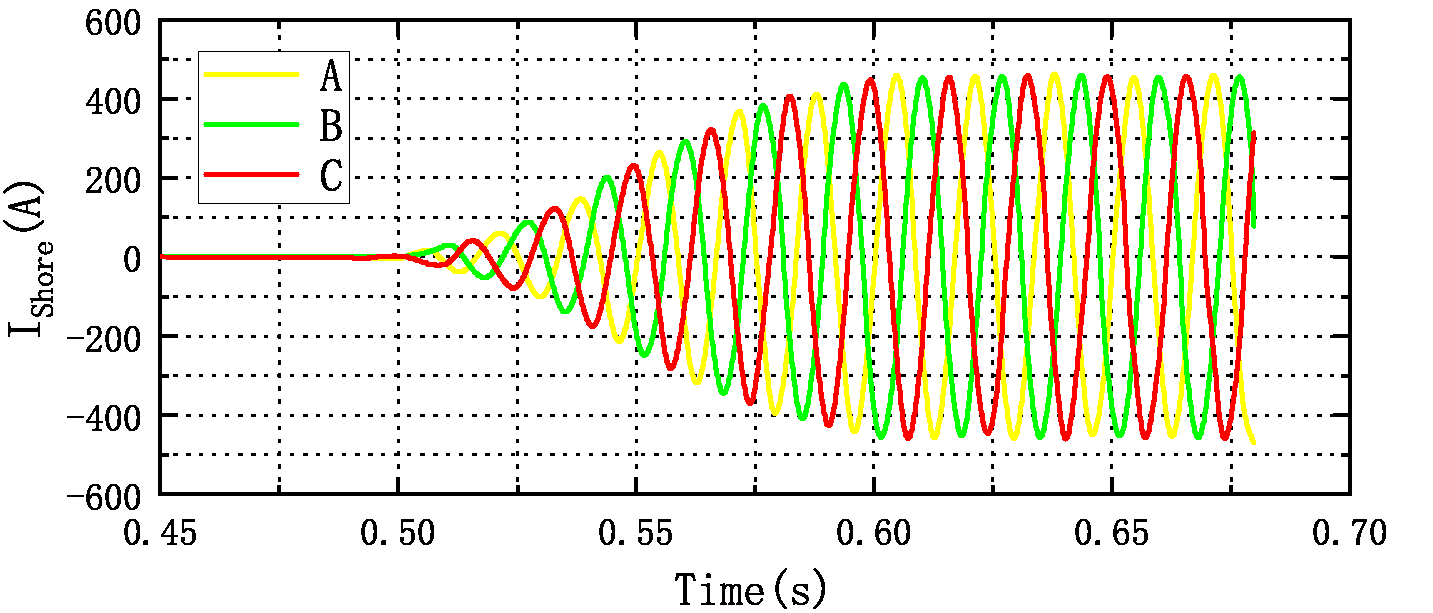
\includegraphics[width=0.9\textwidth]{chapter4/并网/并网过程岸电电流.pdf}
	\caption{船舶岸电并网时电流变化情况}
	\label{fig:船舶岸电并网时电流变化情况}
\end{figure}

\begin{figure}[!htp]
	\centering
	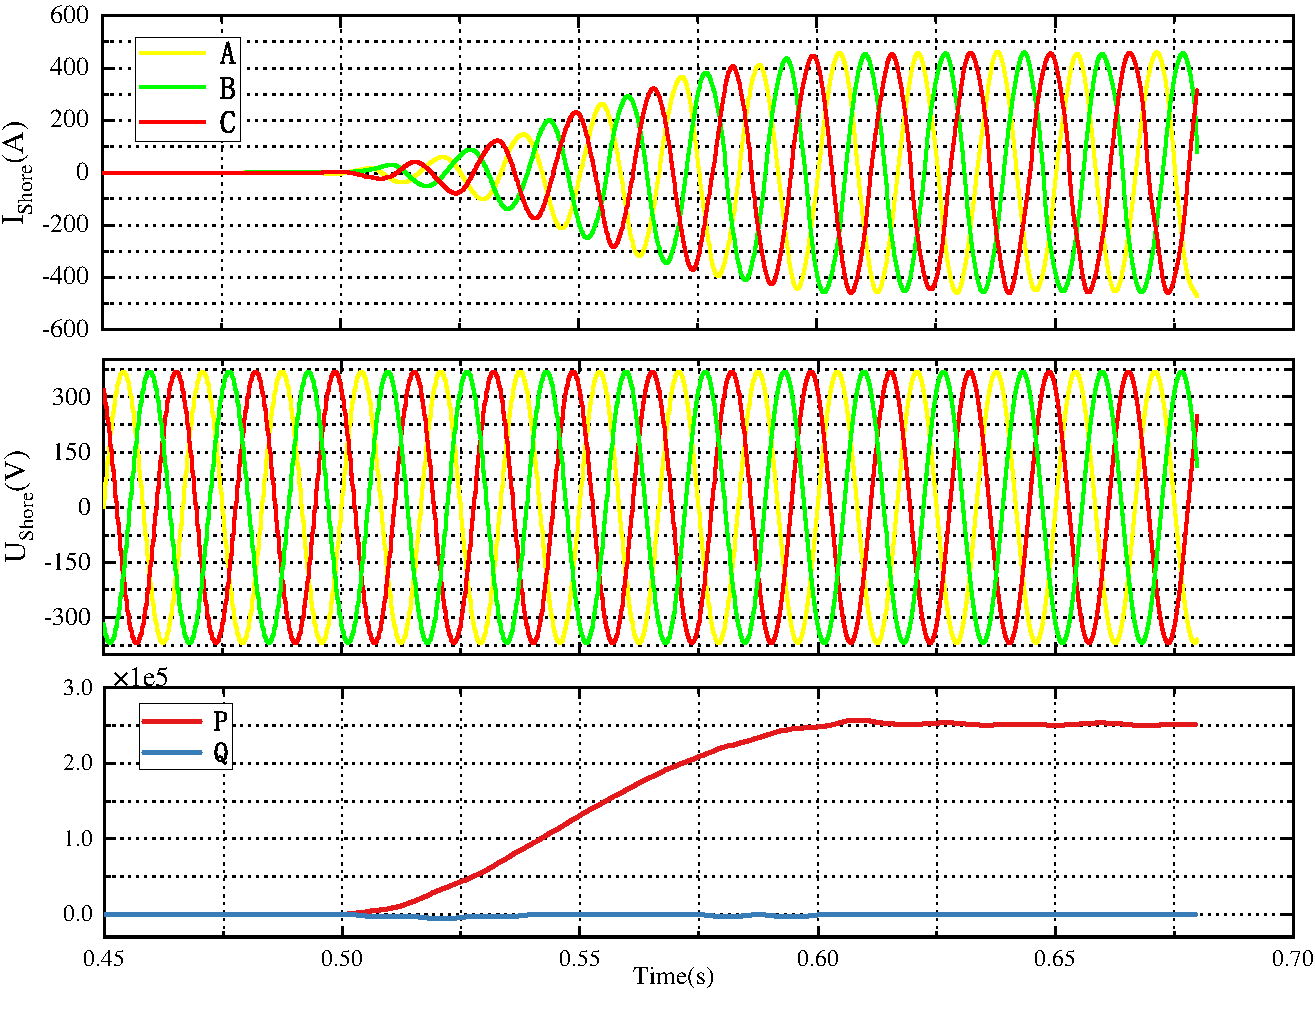
\includegraphics[width=0.9\textwidth]{chapter4/并网/岸电并网情况.pdf}
	\caption{船舶岸电并网情况}
	\label{fig:船舶岸电并网情况}
\end{figure}

\begin{figure}[!htp]
	\centering
	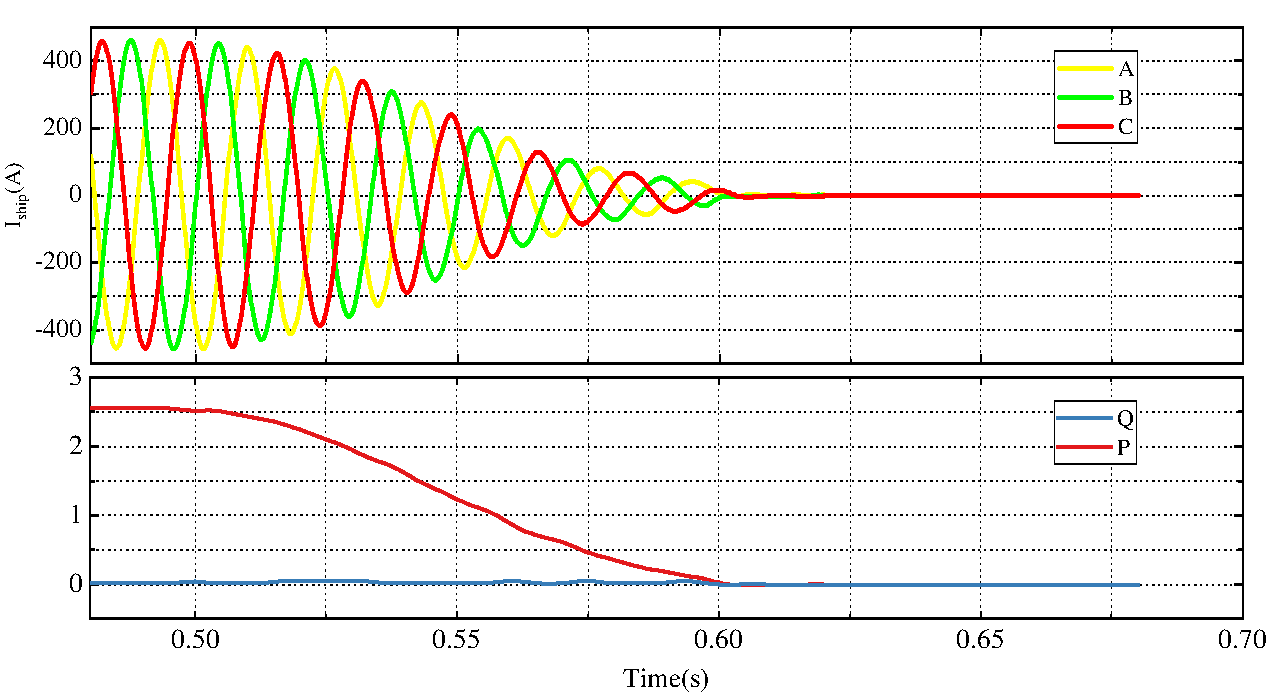
\includegraphics[width=0.9\textwidth]{chapter4/并网/并网船舶发电机情况.pdf}
	\caption{船舶发电机并网情况}
	\label{fig:船舶发电机并网情况}
\end{figure}


\subsection{岸电解列船舶电网过程}



\section{船岸连接系统并网与解列控制方法}

\subsection{基于同步旋转坐标系的锁相环设计}

\subsection{负载转移过程控制与分析}

\begin{table}[!htp]
	\centering
	\caption[电压和频率波动表]{电压和频率波动表\cite{SP7}}
	\label{tab:电压和频率波动表}
	\resizebox{0.9\textwidth}{!}{%
	\begin{tabular}{c}
		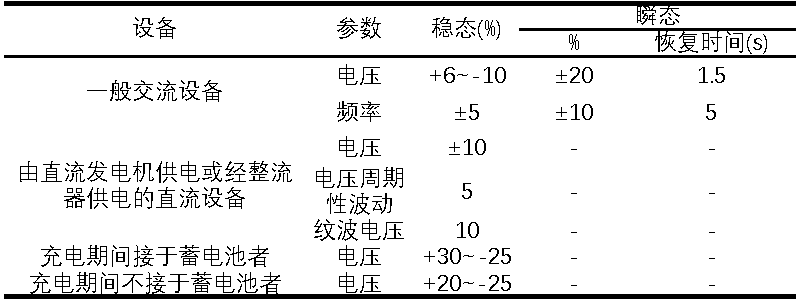
\includegraphics{chapter4/电压和频率波动表.pdf} 
	\end{tabular}
	}
\end{table}

\section{船岸连接系统并网与解列仿真}




\section{本章小结}




